\documentclass{article}

\usepackage{graphicx}
\usepackage{placeins}
\usepackage{fancyhdr}
\usepackage{longtable}
\usepackage{lastpage}
\usepackage{rotating}

% clear the default headers
\fancyhead{}
\fancyfoot{}

\renewcommand{\headrulewidth}{0pt}
\renewcommand{\footrulewidth}{0pt}

\newcommand{\projName}{APO Chapter Organization Website}
\newcommand{\docName}{Software Requirements Document}
\newcommand{\docVersion}{Version 1.0}
\newcommand{\docDate}{October 1, 2012}
\newcommand{\req}[1]{REQ-{#1}}

\setlength\LTleft{0pt}
\setlength\LTright{0pt}



\fancypagestyle{plain}{

\headheight=10mm
\fancyhead{\begin{longtable}{@{\extracolsep{\fill}}|c|c|}
\hline
\projName & \docVersion \\ \hline
\docName & \docDate \\ \hline
\end{longtable}}

 \fancyfoot[C]{\footnotesize Page \thepage\ of \pageref{LastPage}}
}

\pagestyle{plain}

\setcounter{tocdepth}{2}


\title{\projName \\ \vspace{10 mm}
\docName \\\vspace{10 mm}
Devin Schwab\\
Jon Chan}

\date{\docDate}

\begin{document}

\maketitle

\newpage

\tableofcontents
\listoffigures

\newpage

\section{Introduction}
\subsection{Purpose}

\indent\indent This document contains the software requirements for the \projName. This website
will be used by Case's Theta Upsilon chapter of the national service fraternity Alpha Phi Omega (APO).
The website will be accessible via the internet meaning people who are not members will be able to access
the website. In this case the website will simply act as a group of static pages providing basic information.
The actual functionality of the website will be for general members (known as brothers), people currently joining (known as pledges) and members that are elected and appointed to run the chapter (known as exec members).

The requirements in the this document are designed to produce a system that will increase brother interest
in the chapter as well as to decrease the amount of time spent administering the chapter. Additional benefits will
potentially include more transparency and accountability between elected members and general members.

The chapter currently has a website located at http://apo.case.edu, however, based on a survey of members within
the chapter there have been numerous complaints and feature requests. The previous website was built many years ago
and has been maintained by many different people over the years. The updates and fixes to the code base have varied in
quality. This has lead to a difficult to maintain code base. For this reason a new website is being designed with the new
requested features in mind. Many of the requirements in this document have been derived either from the functionality
of the previous website or from feature requests directly from members of the chapter.

\subsection{Scope}

This requirements document deals only with requirements for the \projName. The \projName \,may interface with
other outside pieces of software. In this case the requirements attempt to specify the functionality the outside service has
while remaining general so that outside services can be switched out.

This document is aimed at developers, however, the use cases and project descriptions do provide a high level
description of the project.

\subsection{Document Conventions}

In this document requirements start are labeled in the following
format REQ-\#  where ``\#'' is a number.
The number in the requirement may be followed by a ``.'' and 
another number giving the requirement the form
REQ-\#.\#  This form indicates that the requirement is a
subrequirement of the first number in the requirement. 
Requirements can include any number of numbers and periods.

For example requirement 1 would be labeled \req{1} \,. The first
requirement derived from this requirement it would be labeled\req{1.1}
\,. The first requirement derived from \req{1.1} would be labeled
\req{1.1.1} \,. The number of numbers reflect how deep the requirement
is and the ordering reflects where a requirement was derived from.

Features are referred to as FE-\# where ``\#'' is a number.

\subsection{Definitions}

% Add definition to the table
\begin{longtable}{lp{8cm}}

{\bf Brother} & A general member of the chapter that has gone through
the pledging process. \\ \\
{\bf Contract} & The requirements that a member must satisfy to remain
in good standing with the chapter \\ \\
{\bf Exec Member} & A general member of the chapter (brother) that is
elected or appointed to run a specific aspect of the chapter. \\ \\
{\bf Membership Review} & Event at the end of the semester in which
the completion of each member's contract is reviewed by the chapter\\ \\
{\bf Pledge} & A member who has completed the initiation ceremony, but
not the induction ceremony. These members do not have the full
privilege of a brother\\ \\
{\bf Rushee} & A person who is interested in joining APO, but is not
yet a pledge \\ \\
{\bf Service Report} & Request for approval of community service hours
\\ \\

\end{longtable}

\section{Overall Description}

\subsection{Project Features}

\subsection{User Classes and Characteristics}

This project has 3 main classes of users:

\begin{enumerate}
  \item Exec Members
  \item Brothers and Pledges
  \item Rushee
\end{enumerate}

Each of these user classes is described in more detail in the next sections

\subsubsection{Exec Members}

These users have been elected or appointed by the chapter to run some
part of the chapter. All Exec members must also be a Brother. Exec
members have access the administrative tools of the \projName \,. One
of the goals of this project is to decrease the amount of time that
exec members spend administering the chapter.

\subsubsection{Brothers and Pledges}

This user class can be split into two subclasses. Brothers have been
inducted into the chapter, whereas pledges have not. In the actual
workings of the chapter brothers have more rights than pledges, such
as voting. However, from the perspective of this project the only
difference between brothers and pledges is the information displayed
by each of the features.

\subsubsection{Rushee}

This user class consists of potential members. These users will only
have access to informational features.

\subsection{Operating Environment}

\subsubsection{Website Operating Environment}

The website shall be capable of running on any platform which provides
an HTTP webserver. The webserver must also provide a way for scripting
responses to web requests in order to make the website respond to user
input and previously stored information.

\subsubsection{User Operating Environment}

The user shall be capable of accessing the website from any modern
browser. This includes mobile devices.

\subsection{Assumptions and Dependencies}

The website depends on a working webserver and a working internet
connection.

\section{System Features and Associated Requirements}

\subsection{General Requirements}

\begin{tabular}{lp{8cm}}
\req{1} & The user shall be able to login with a username and password\\
\req{1.1} & The website shall accept a password of any length greater than 8 characters long\\
\req{1.2} & The website shall guarantee that each user's username is
unique\\
\end{tabular}

\subsection{FE-1: Create, update, track, and report service events and
  hours}

\subsubsection{Use case Diagram}

\newpage

\FloatBarrier
\begin{sidewaysfigure}[h]
\centering
\caption{Exec Use Case Flowchart for FE-1}
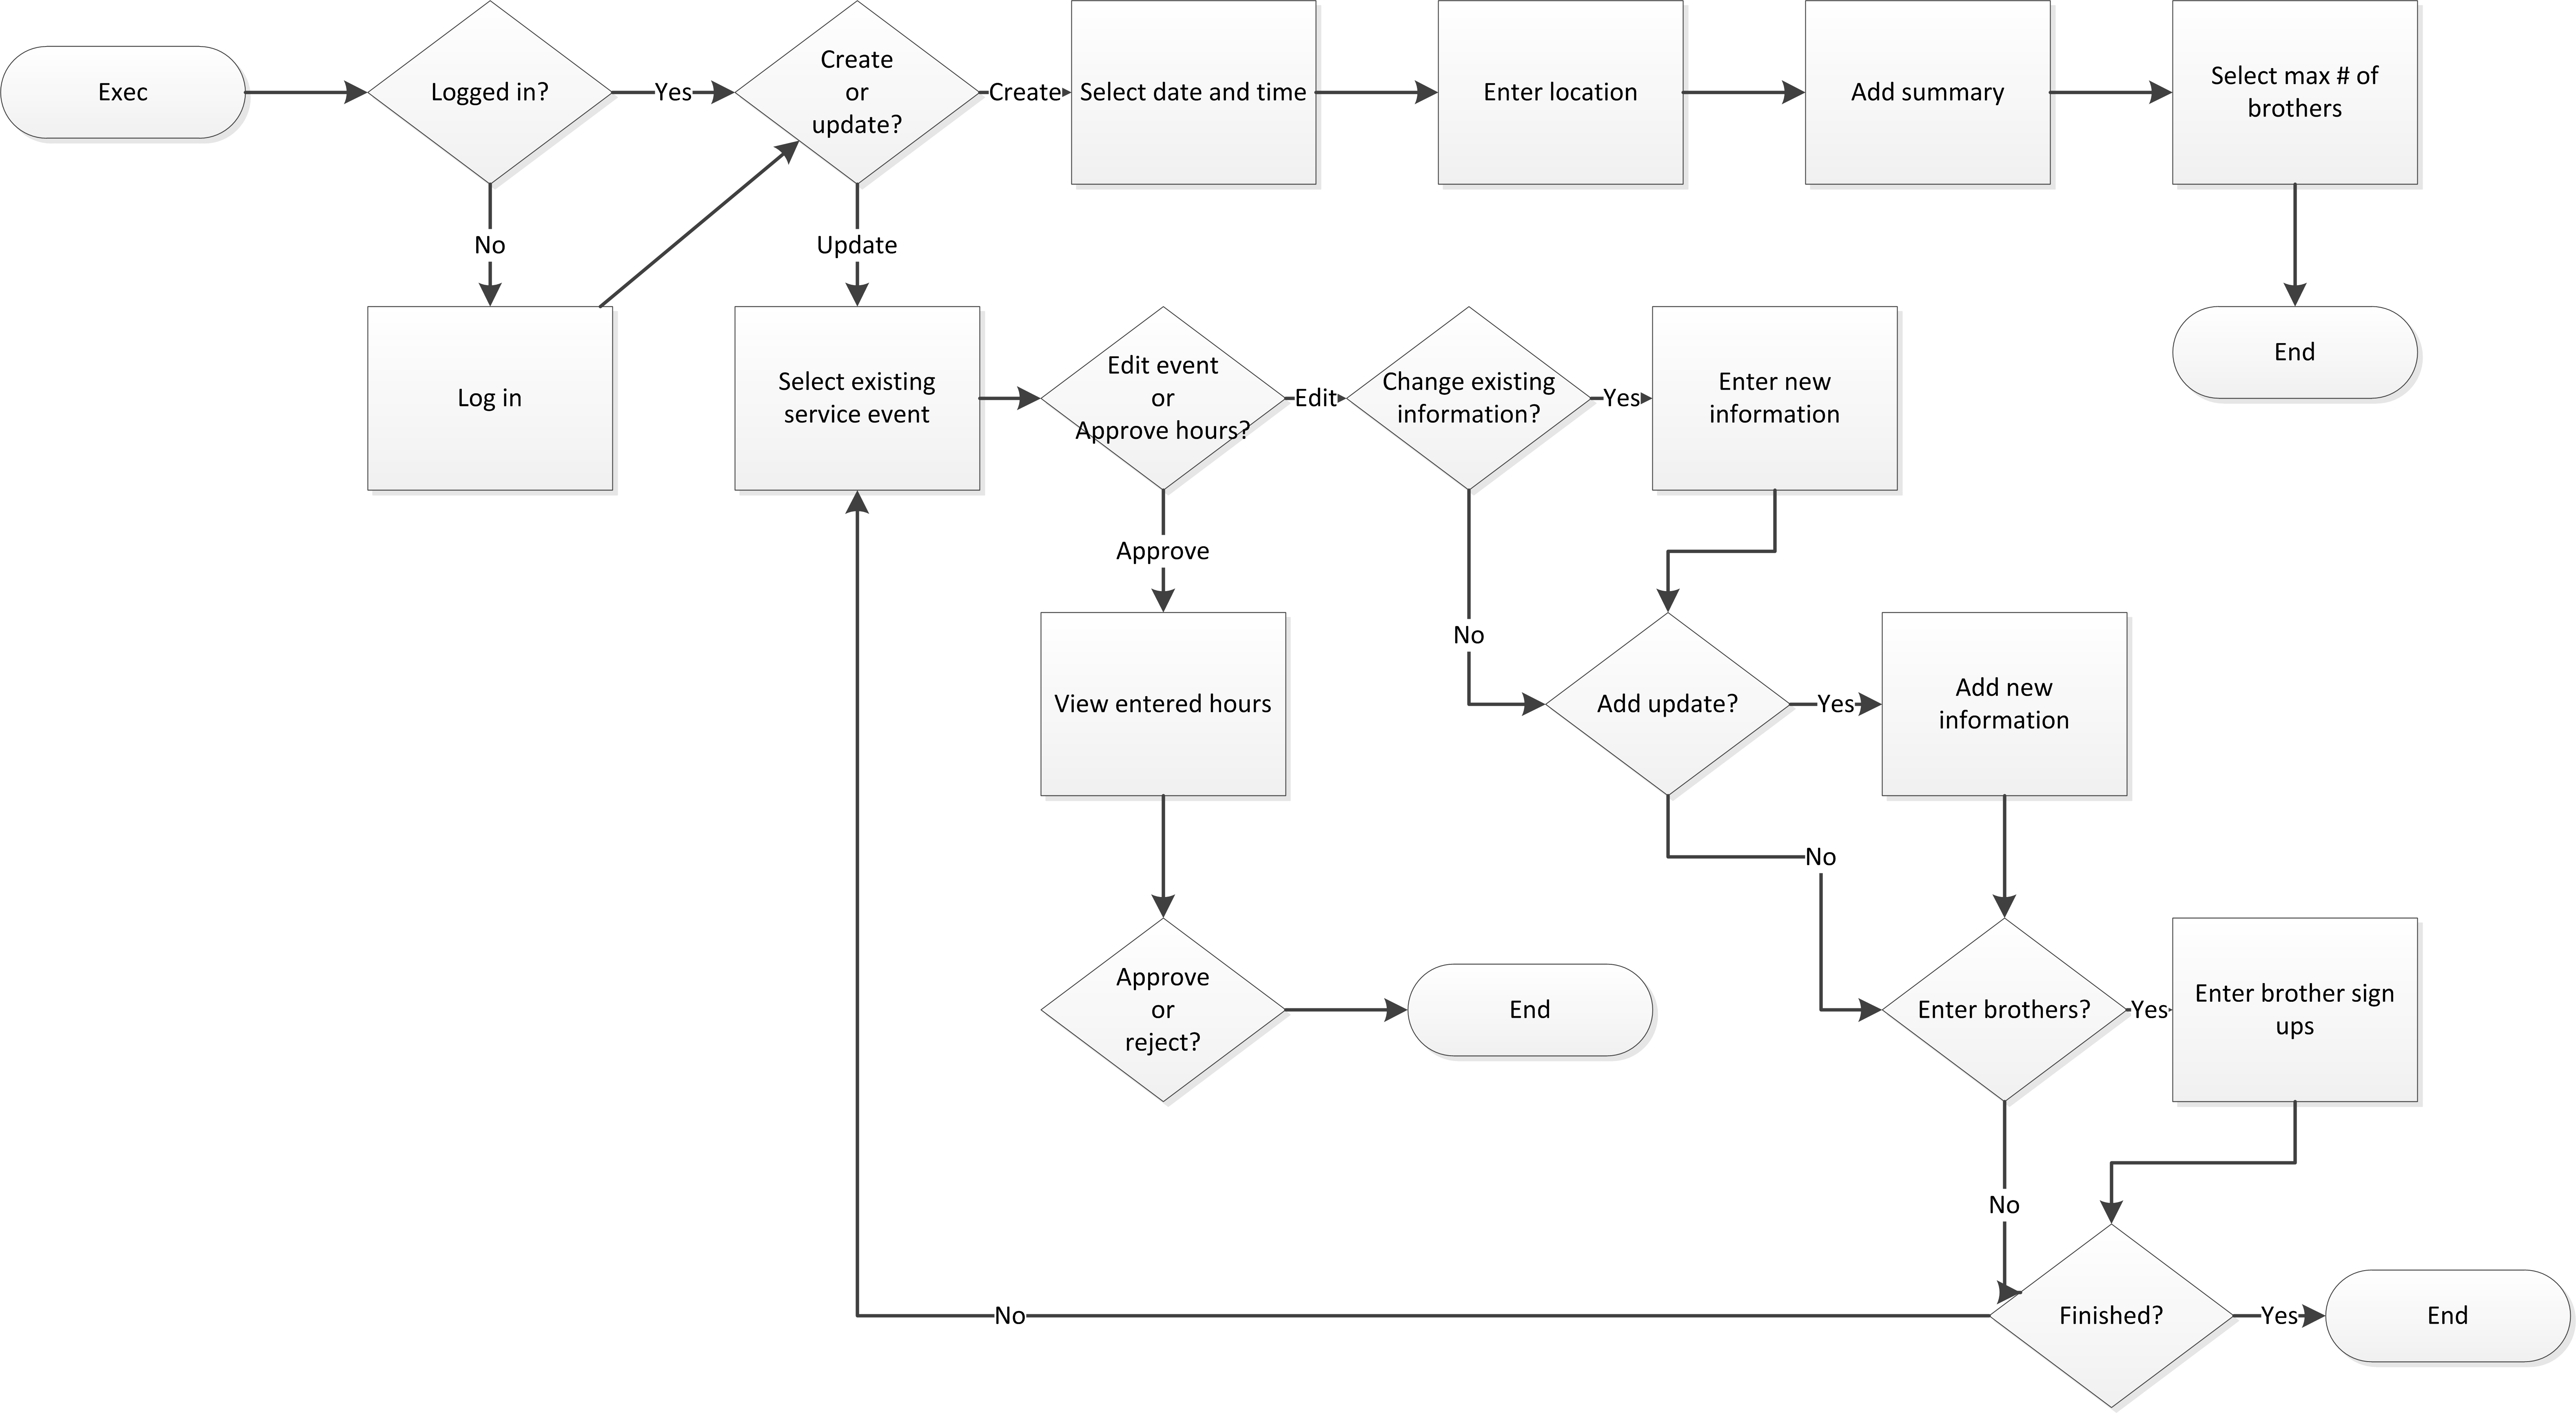
\includegraphics[scale=.75]{img/execUseCaseFE1.png}
\label{fig:execUseCaseFE1}
\end{sidewaysfigure}
\FloatBarrier

\newpage

\newpage

\FloatBarrier
\begin{sidewaysfigure}[h]
\centering
\caption{Brother/Pledge Use Case Flowchart for FE-1}
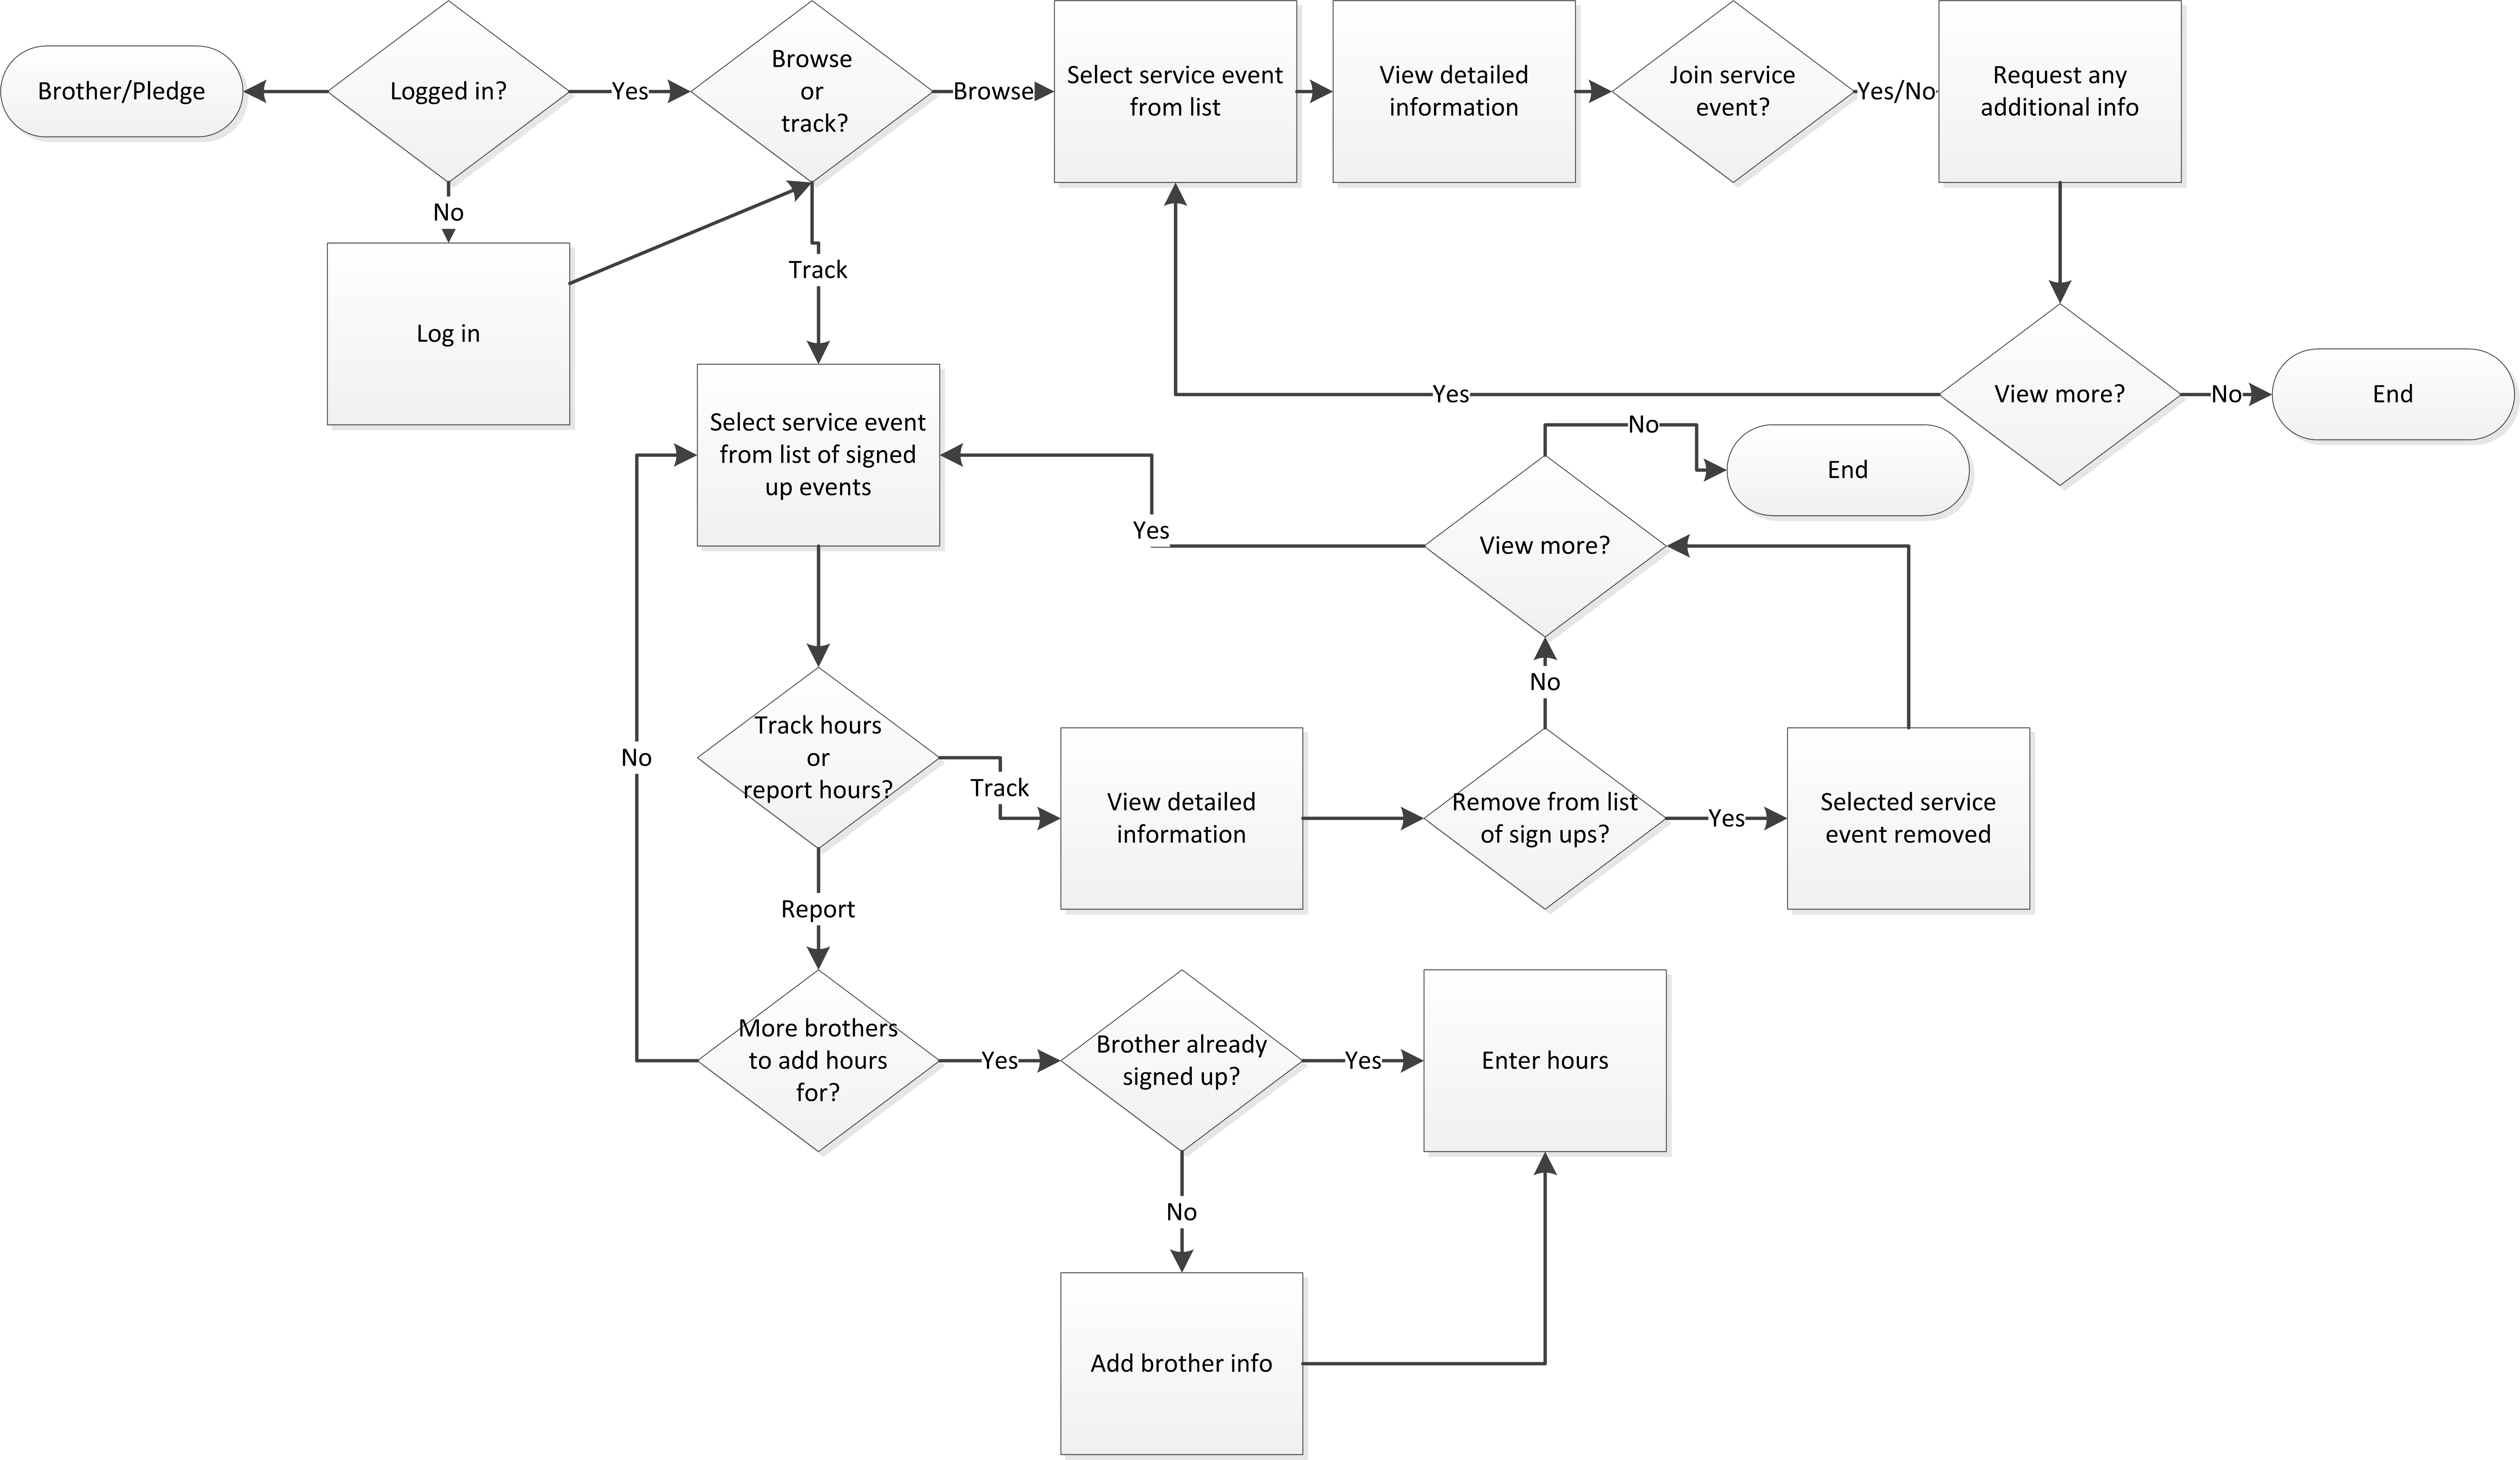
\includegraphics[scale=.75]{img/brotherUseCaseFE1.png}
\label{fig:brotherUseCaseFE1}
\end{sidewaysfigure}
\FloatBarrier

\newpage

\subsubsection{Requirements}

\begin{tabular}{lp{8cm}}
\req{2} & Exec members shall be able to create a service event \\
\req{2.1} & Exec members shall be able to enter a date and time for an
event\\
\req{2.2} & Exec members shall be able to enter a location for an
event\\
\req{2.3} & Exec members shall be able to enter an event description
\\
\req{2.4} & Exec members shall be able to specify the maximum number
of brothers that can attend the event\\
\req{2.5} & Exec members shall be able to specify any other additional
information necessary \\
\req{2.6} & Exec members shall be able to require brothers and pledges
to enter in
additional information\\
\req{3} & Exec members shall be able to update existing service events
\\
\req{3.1} & Exec members shall be able to update the date and time for an
event\\
\req{3.2} & Exec members shall be able to update the location for an
event\\
\req{3.3} & Exec members shall be able to update the event description
\\
\req{3.4} & Exec members shall be able to update the maximum number
of brothers that can attend the event\\
\req{3.5} & Exec members shall be able to update any other additional
information necessary \\
\req{3.6} & Exec members shall be able to update the additional
information required from brothers and pledges\\
\req{4} & Brothers and pledges shall be able to view existing service
events \\
\req{4.1} & Brothers and pledges shall be able to view the date and time for an
event\\
\req{4.2} & Brothers and pledges shall be able to view the location for an
event\\
\req{4.3} & Brothers and pledges shall be able to view the event description
\\
\req{4.4} & Brothers and pledges shall be able to view the maximum number
of brothers that can attend the event\\
\req{4.5} & Brothers and pledges shall be able to view any other additional
information necessary \\
\req{4.6} & Brothers and pledges shall be able to view their answers
to the additional information requested\\
\req{5} & Brothers and pledges shall be able to update their responses
to the additional information requested\\
\req{6} & Brothers and pledges shall be able to join existing service
events \\
\req{7} & Brothers and pledges shall be able to report service hours
for a service event \\
\req{7.1} & Brothers and pledges shall be able to enter in the names
of all brothers and pledges who participated in the event\\
\req{7.2} & Brothers and pledges shall be able to enter the number of
hours of participation for
each brother and pledge who participated in the event\\
\req{8} & Exec members shall be able to approve submitted service
hours\\
\req{8.1} & Exec members shall be able to view each brother or pledge who was
submitted as participating in the event\\
\req{8.2} & Exec members shall be able to view the hours of each brother
or pledge
who was  submitted as participating in the event\\
\req{8.3} & Exec members shall be able to approve or reject the hours
of each brother who was submitted as participating in the event\\
\end{tabular}

\subsection{FE-2: Create, update, sign and track progress of member
  contracts}

\subsubsection{Use case Diagram}

\newpage

\FloatBarrier
\begin{sidewaysfigure}[h]
\centering
\caption{Exec Use Case Flowchart for FE-2}
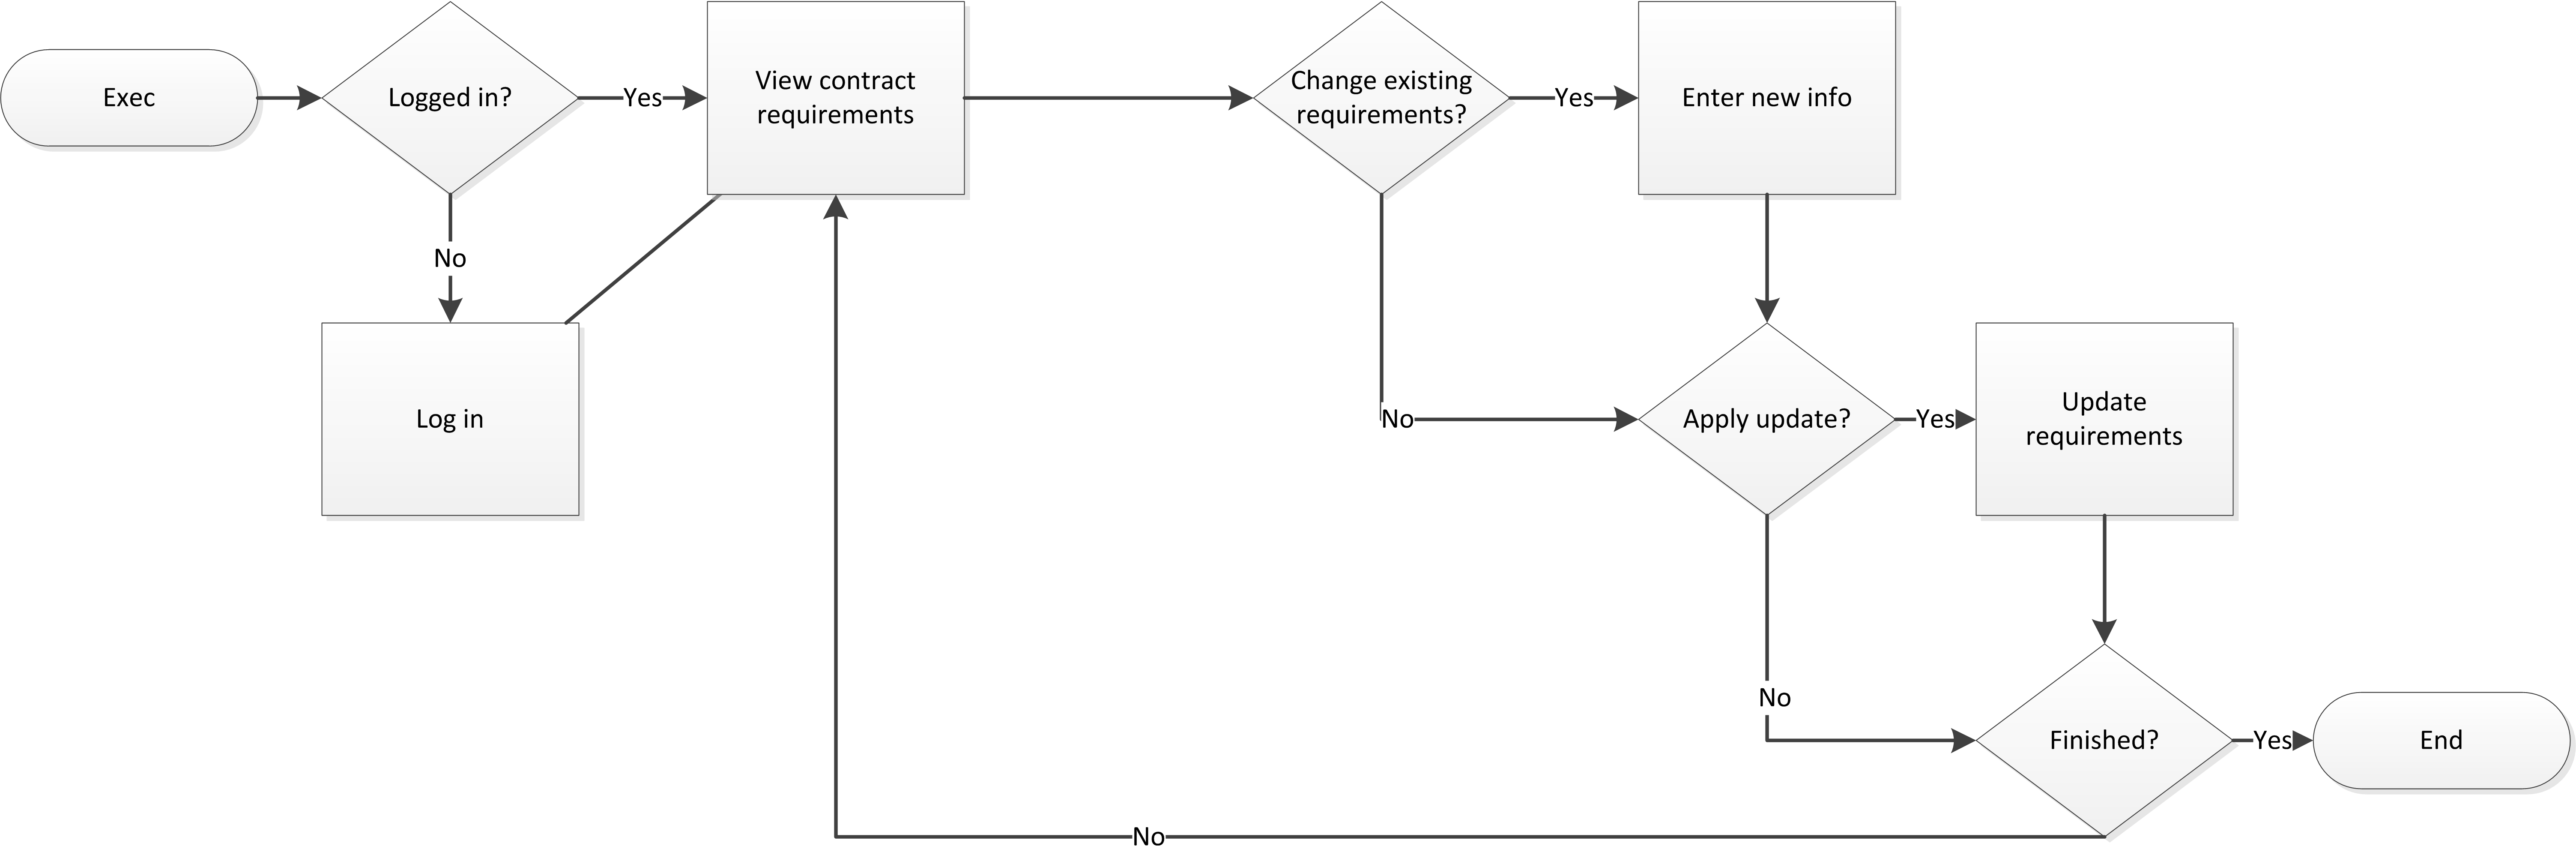
\includegraphics[scale=.75]{img/execUseCaseFE2.png}
\label{fig:execUseCaseFE2}
\end{sidewaysfigure}
\FloatBarrier

\newpage

\subsubsection{Requirements}

\begin{tabular}{lp{8cm}}
\req{9} & Exec members shall be able to create new contract types \\
\req{9.1} & Exec members shall be able to specify requirements based
on service hours completed\\
\req{9.2} & Exec members shall be able to specify requirements based
on membership dues\\
\req{9.3} & Exec members shall be able to specify requirements based
on attendance at events\\
\req{10} & All members shall be able to view existing contract types\\
\req{10.1} & All members shall be able to view the service hour
contract requirements for each contract type\\
\req{10.2} & All members shall be able to view the membership dues
contract requirements for each contract type\\
\req{10.3} & All members shall be able to view the attendance based
contract requirements for each contract type\\
\req{11} & Exec members shall be able to edit contract requirements for
each contract type \\
\req{11.1} & Exec members shall be able to update requirements based
on service hours completed\\
\req{11.2} & Exec members shall be able to update requirements based
on membership dues\\
\req{11.3} & Exec members shall be able to update requirements based
on attendance at events\\
\req{12} & Brothers and pledges shall be able to sign a contract \\
\req{13} & Brothers and pledges shall be able to view their contract
progress\\
\req{13.1} & Brothers and pledges shall be able to view progress of completion
of requirements based
on service hours completed for the contract type they have signed\\
\req{13.2} & Brothers and pledges shall be able to view progress of completion
of requirements based
on membership dues for the contract type they have signed\\
\req{13.3} & Brothers and pledges shall be able to view progress of completion
of requirements based
on attendance at events for the contract type they have signed\\
\req{14} & Exec members shall be able to view everyone's contract
progress \\
\req{14.1} & Exec members shall be able to view progress of completion
of requirements based
on service hours completed\\
\req{14.2} & Exec membersshall be able to view progress of completion
of requirements based
on attendance at events\\
\req{14.3} & Exec members  Brothers and pledges shall be able to view progress of completion
of requirements based
on membership dues\\
\req{15} & Exec members shall be able to review incomplete contracts
and manually pass them 
\\
\end{tabular}

\subsection{FE-3: Create, update and view profiles of members and
  alumni}

\subsubsection{Use case Diagram}

\newpage

\FloatBarrier
\begin{sidewaysfigure}[h]
\centering
\caption{Exec Use Case Flowchart for FE-3}
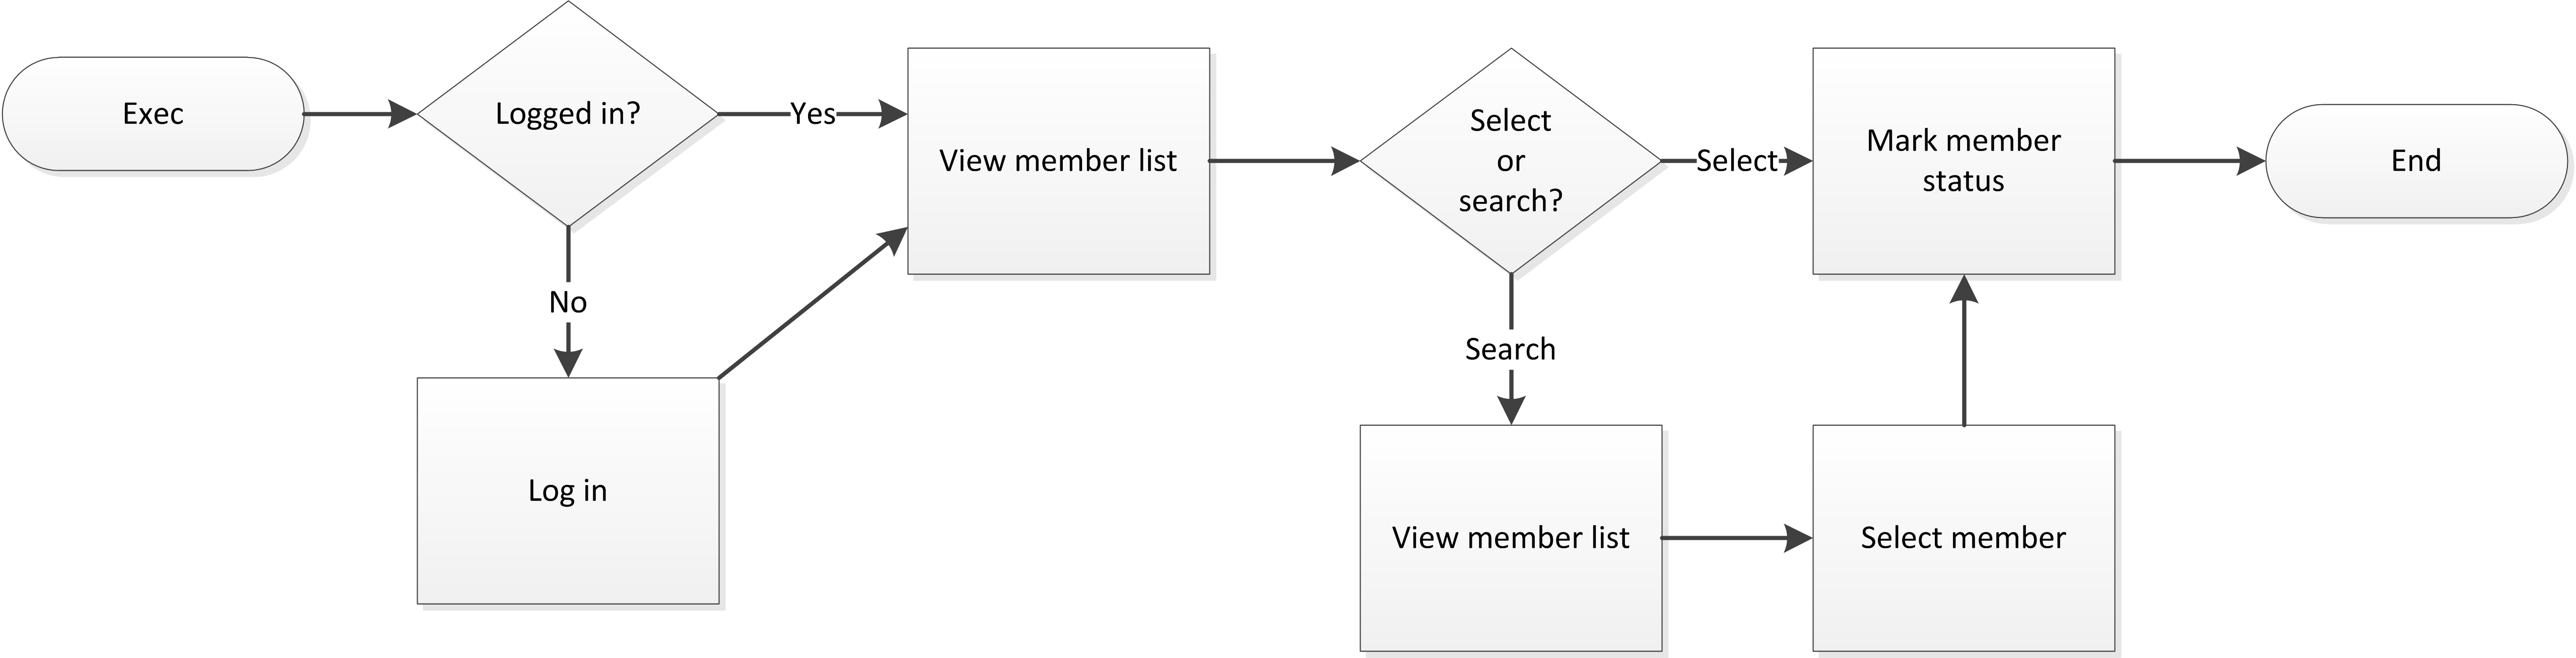
\includegraphics[scale=.75]{img/execUseCaseFE3.png}
\label{fig:execUseCaseFE3}
\end{sidewaysfigure}
\FloatBarrier

\newpage

\subsubsection{Requirements}

\begin{tabular}{lp{8cm}}
\req{16} & Exec members shall be able to create member profile types\\
\req{16.1} & Exec members shall be able to name the member profile
types\\
\req{16.2} & Exec members shall be able to assign page permissions for
new profile type\\
\req{17} & Exec members shall be able to create new member accounts\\
\req{17.1} & Exec members shall be able to add a first and last name
to new accounts \\
\req{17.2} & Exec members shall be able to add an address to new
accounts \\
\req{17.3} & Exec members shall be able to add a phone number to new
accounts \\
\req{17.4} & Exec members shall be able to add a profile picture to
new accounts \\
\req{18} & Exec members shall be able to delete member accounts\\
\req{19} & Exec members shall be able to set member profiles to an existing profile type \\
\req{20} & Brothers and pledges shall be able to update the
information in their profiles \\
\req{20.1} & Brothers and pledges shall be able to add a first and last name
to their own accounts \\
\req{20.2} & Brothers and pledges shall be able to add an address to their own
accounts \\
\req{20.3} & Brothers and pledges shall be able to add a phone number to their own
accounts \\
\req{20.4} & Brothers and pledges shall be able to add a profile picture to
their own accounts \\
\req{21} & All members should be able to view other member profiles \\
\req{21.1} & All members shall be able to add a first and last name
to their own accounts \\
\req{21.2} & All members shall be able to add an address to their own
accounts \\
\req{21.3} & All members shall be able to add a phone number to their own
accounts \\
\req{21.4} & All members shall be able to add a profile picture to
their own accounts \\
\end{tabular}

\subsection{FE-4: Update and view chapter calendar}

\subsubsection{Use case Diagram}

\newpage

\FloatBarrier
\begin{sidewaysfigure}[h]
\centering
\caption{Exec Use Case Flowchart for FE-4}
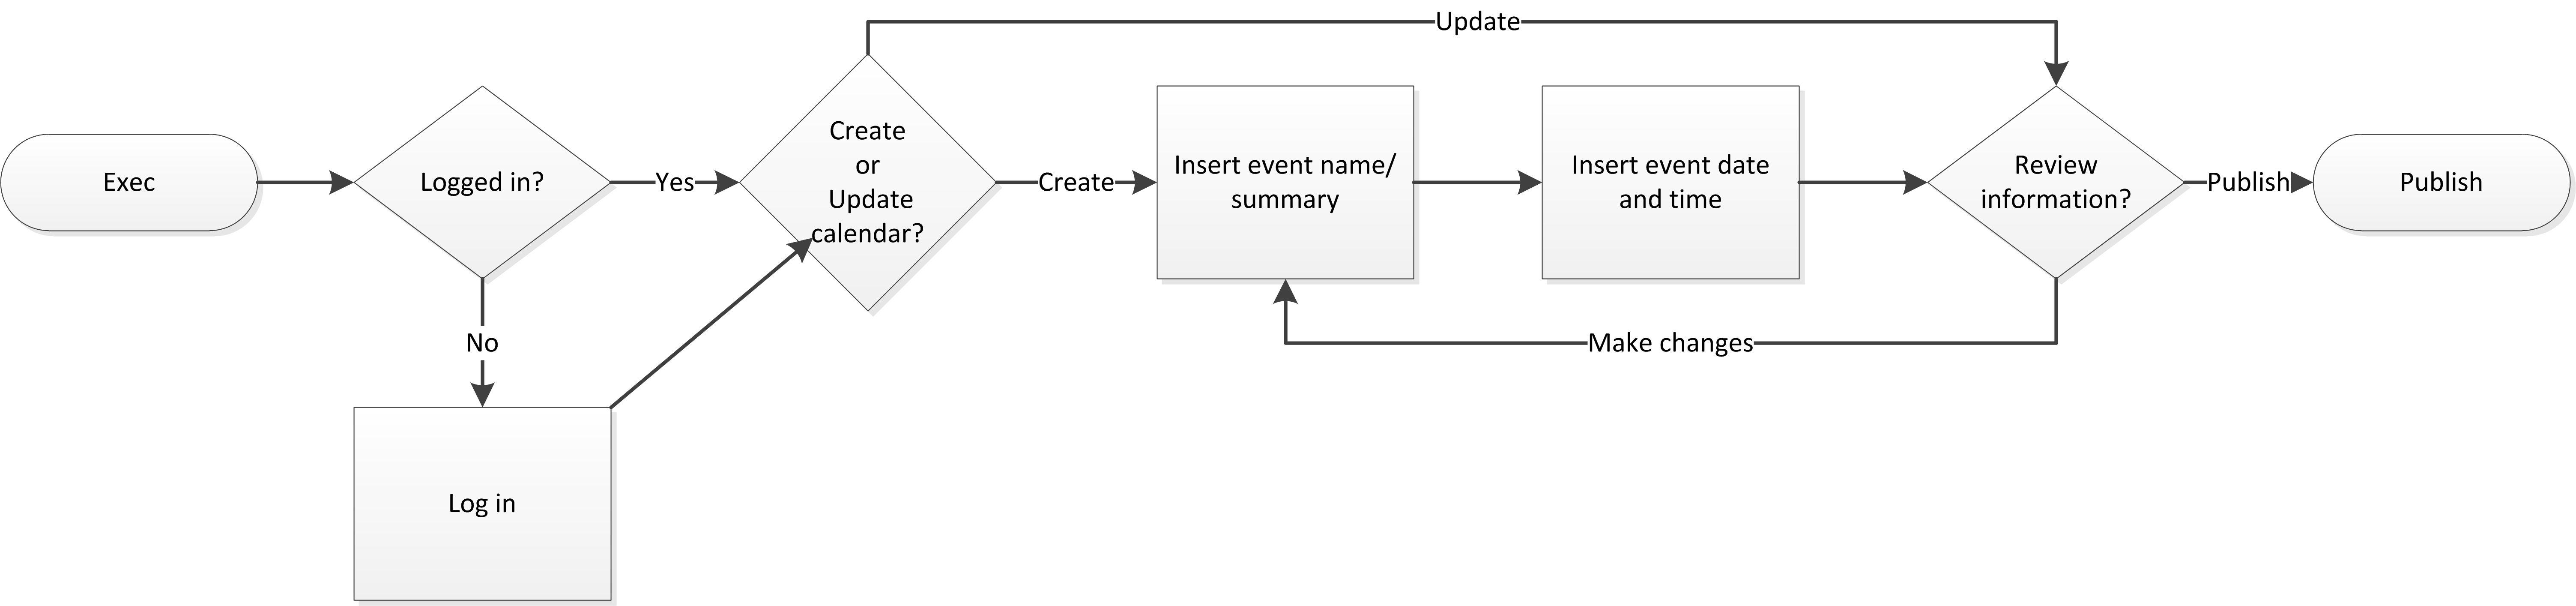
\includegraphics[scale=.75]{img/execUseCaseFE4.png}
\label{fig:execUseCaseFE4}
\end{sidewaysfigure}
\FloatBarrier

\newpage

\subsubsection{Requirements}

\begin{tabular}{lp{8cm}}
\req{22} & Exec shall be able to create new calendar events \\
\req{22.1} & Exec members shall be able to enter a date and time for an
event\\
\req{22.2} & Exec members shall be able to enter a location for an
event\\
\req{22.3} & Exec members shall be able to enter an event description
\\
\req{22.5} & Exec members shall be able to specify any other additional
information necessary \\
\req{23} & Exec shall be able to update existing calendar events \\
\req{23.1} & Exec members shall be able to update the date and time for an
event\\
\req{23.2} & Exec members shall be able to update the location for an
event\\
\req{23.3} & Exec members shall be able to update the event description
\\
\req{23.5} & Exec members shall be able to update any other additional
information necessary \\
\req{24} & Exec shall be able to delete existing calendar events \\
\req{25} & Brothers and pledges shall be able to view calendars \\
\req{26} & Brothers and pledges shall be able to view event details
for events in the calendar\\
\req{26.1} & Brothers and pledges shall be able to view the date and time for an
event\\
\req{26.2} & Brothers and pledges shall be able to view the location for an
event\\
\req{26.3} & Brothers and pledges shall be able to view the event description
\\
\req{26.5} & Brothers and pledges shall be able to view any other additional
information necessary \\
\end{tabular}

\subsection{FE-5: Write and comment on chapter blog}

\subsubsection{Use case Diagram}

\newpage

\FloatBarrier
\begin{sidewaysfigure}[h]
\centering
\caption{Exec Use Case Flowchart for FE-5}
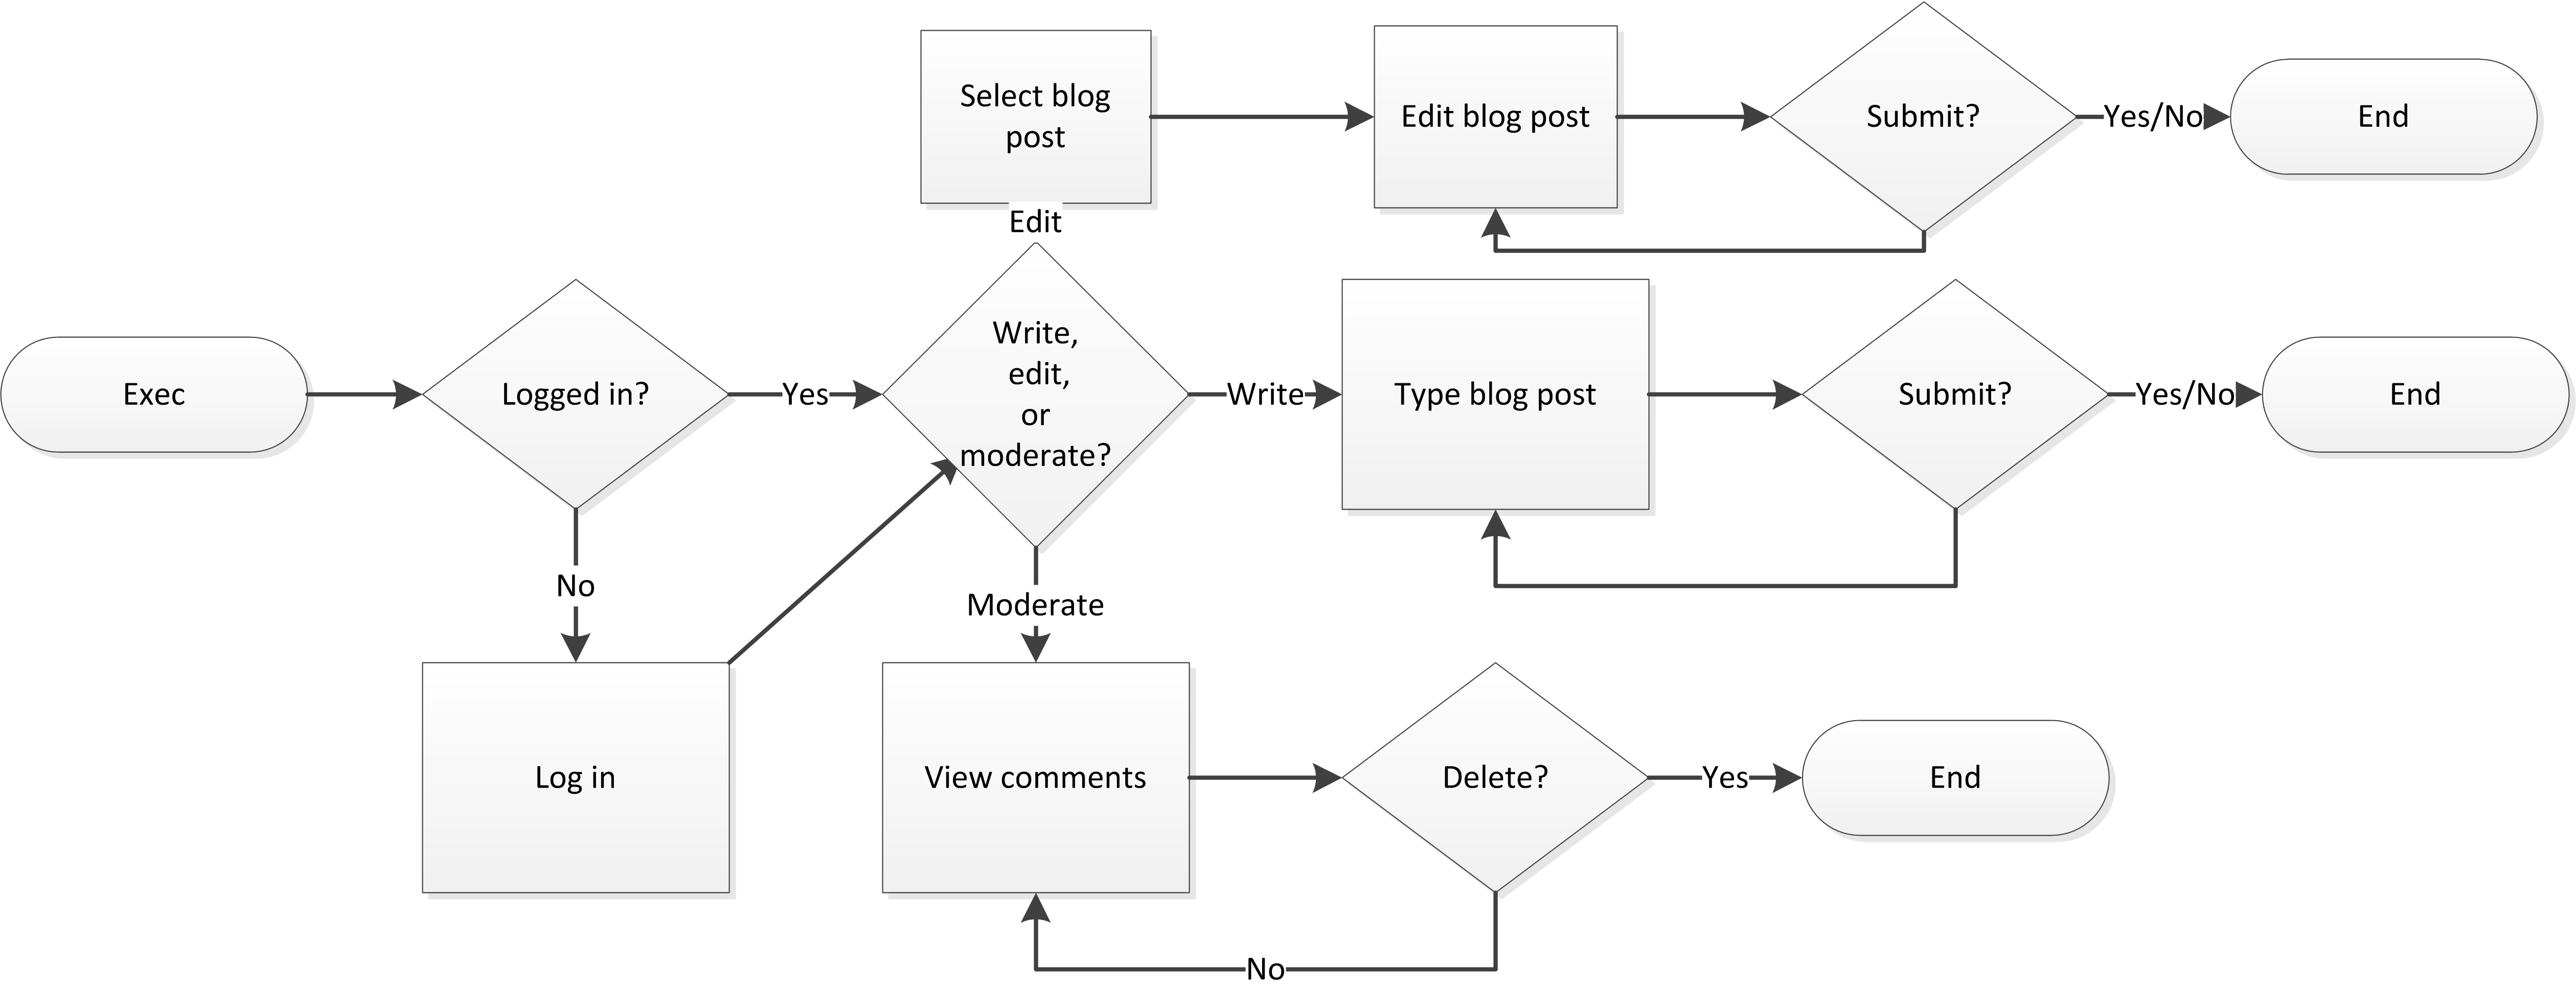
\includegraphics[scale=.75]{img/execUseCaseFE5.png}
\label{fig:execUseCaseFE5}
\end{sidewaysfigure}
\FloatBarrier

\newpage

\subsubsection{Requirements}

\begin{tabular}{lp{8cm}}
\req{27} & Exec members shall be able to write new blog posts \\
\req{28} & Exec members shall be able to edit existing blog posts \\
\req{29} & Exec members shall be able to moderate comments \\
\req{30} & Members and nonmembers will be able to view blog posts \\
\req{31} & Members shall be able to comment on blog posts \\
\end{tabular}

\subsection{FE-6: Submit and view photos of chapter members and
  chapter events}

\subsubsection{Use case Diagram}

\newpage

\FloatBarrier
\begin{sidewaysfigure}[h]
\centering
\caption{Exec Use Case Flowchart for FE-6 - Review Photo Submissions}
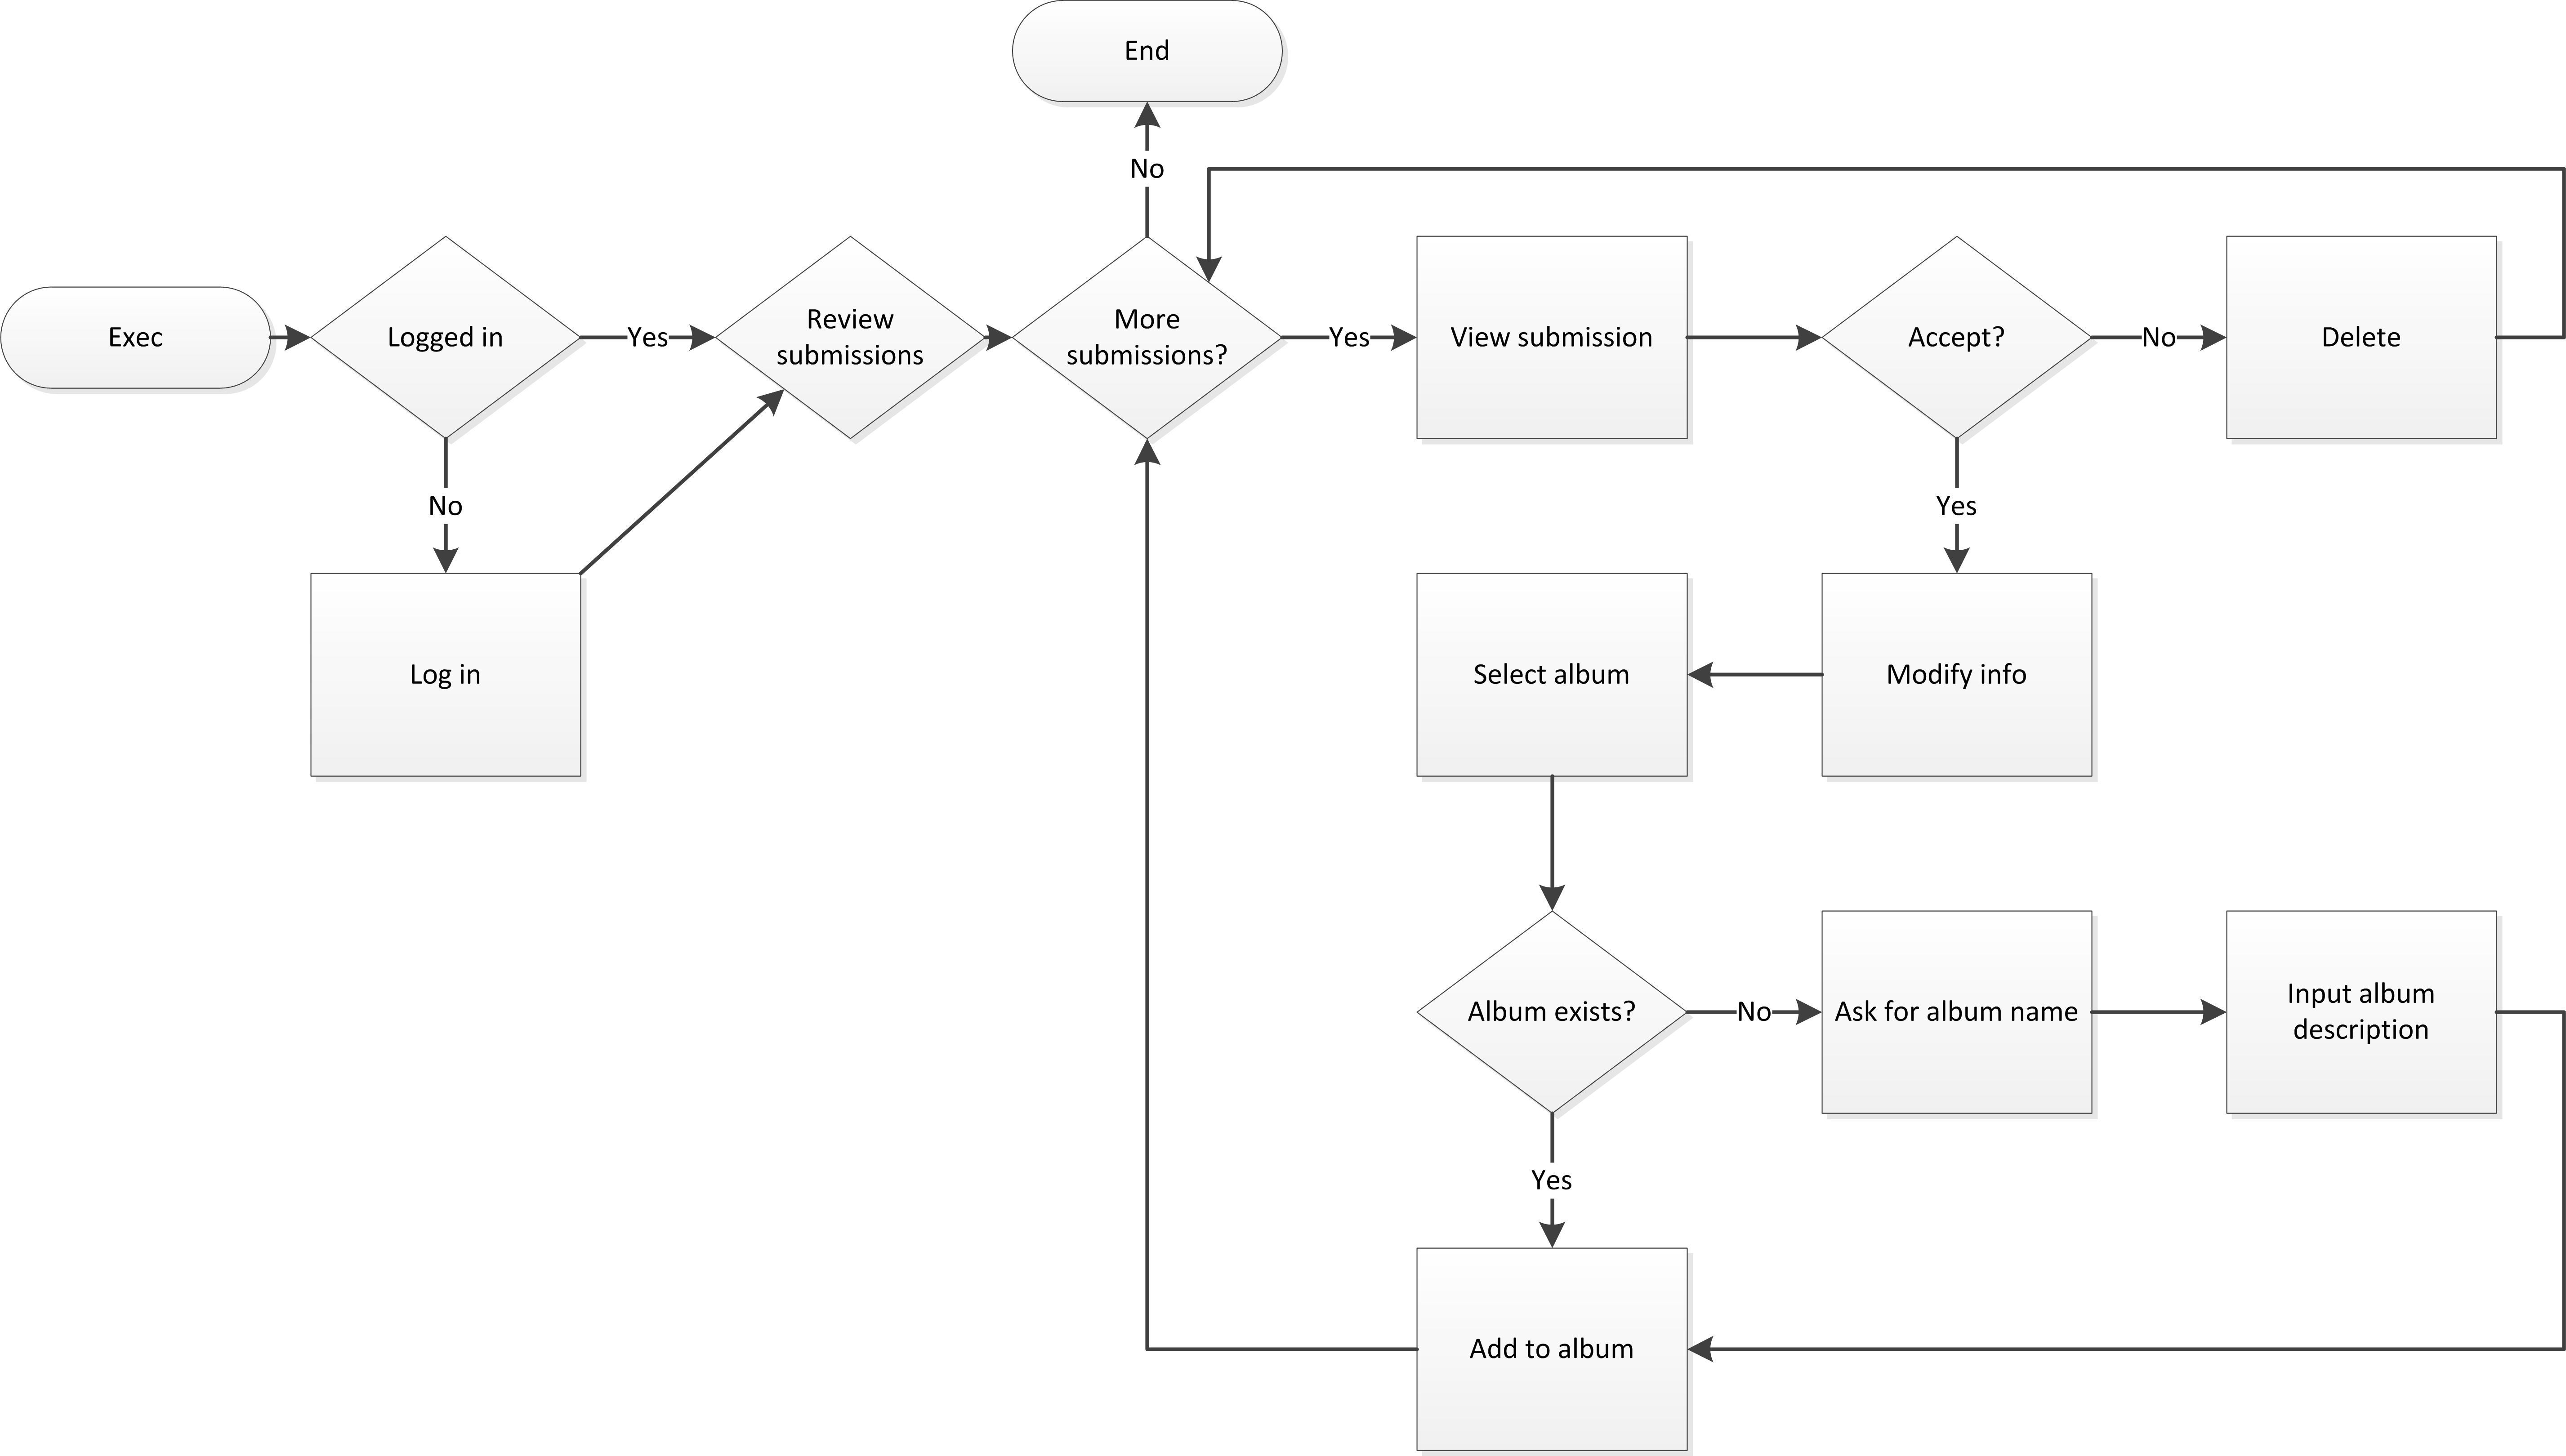
\includegraphics[scale=.75]{img/execUseCaseFE6_review.png}
\label{fig:execUseCaseFE6_review}
\end{sidewaysfigure}
\FloatBarrier

\newpage

\newpage

\FloatBarrier
\begin{sidewaysfigure}[h]
\centering
\caption{Exec Use Case Flowchart for FE-6 - Organize Albums}
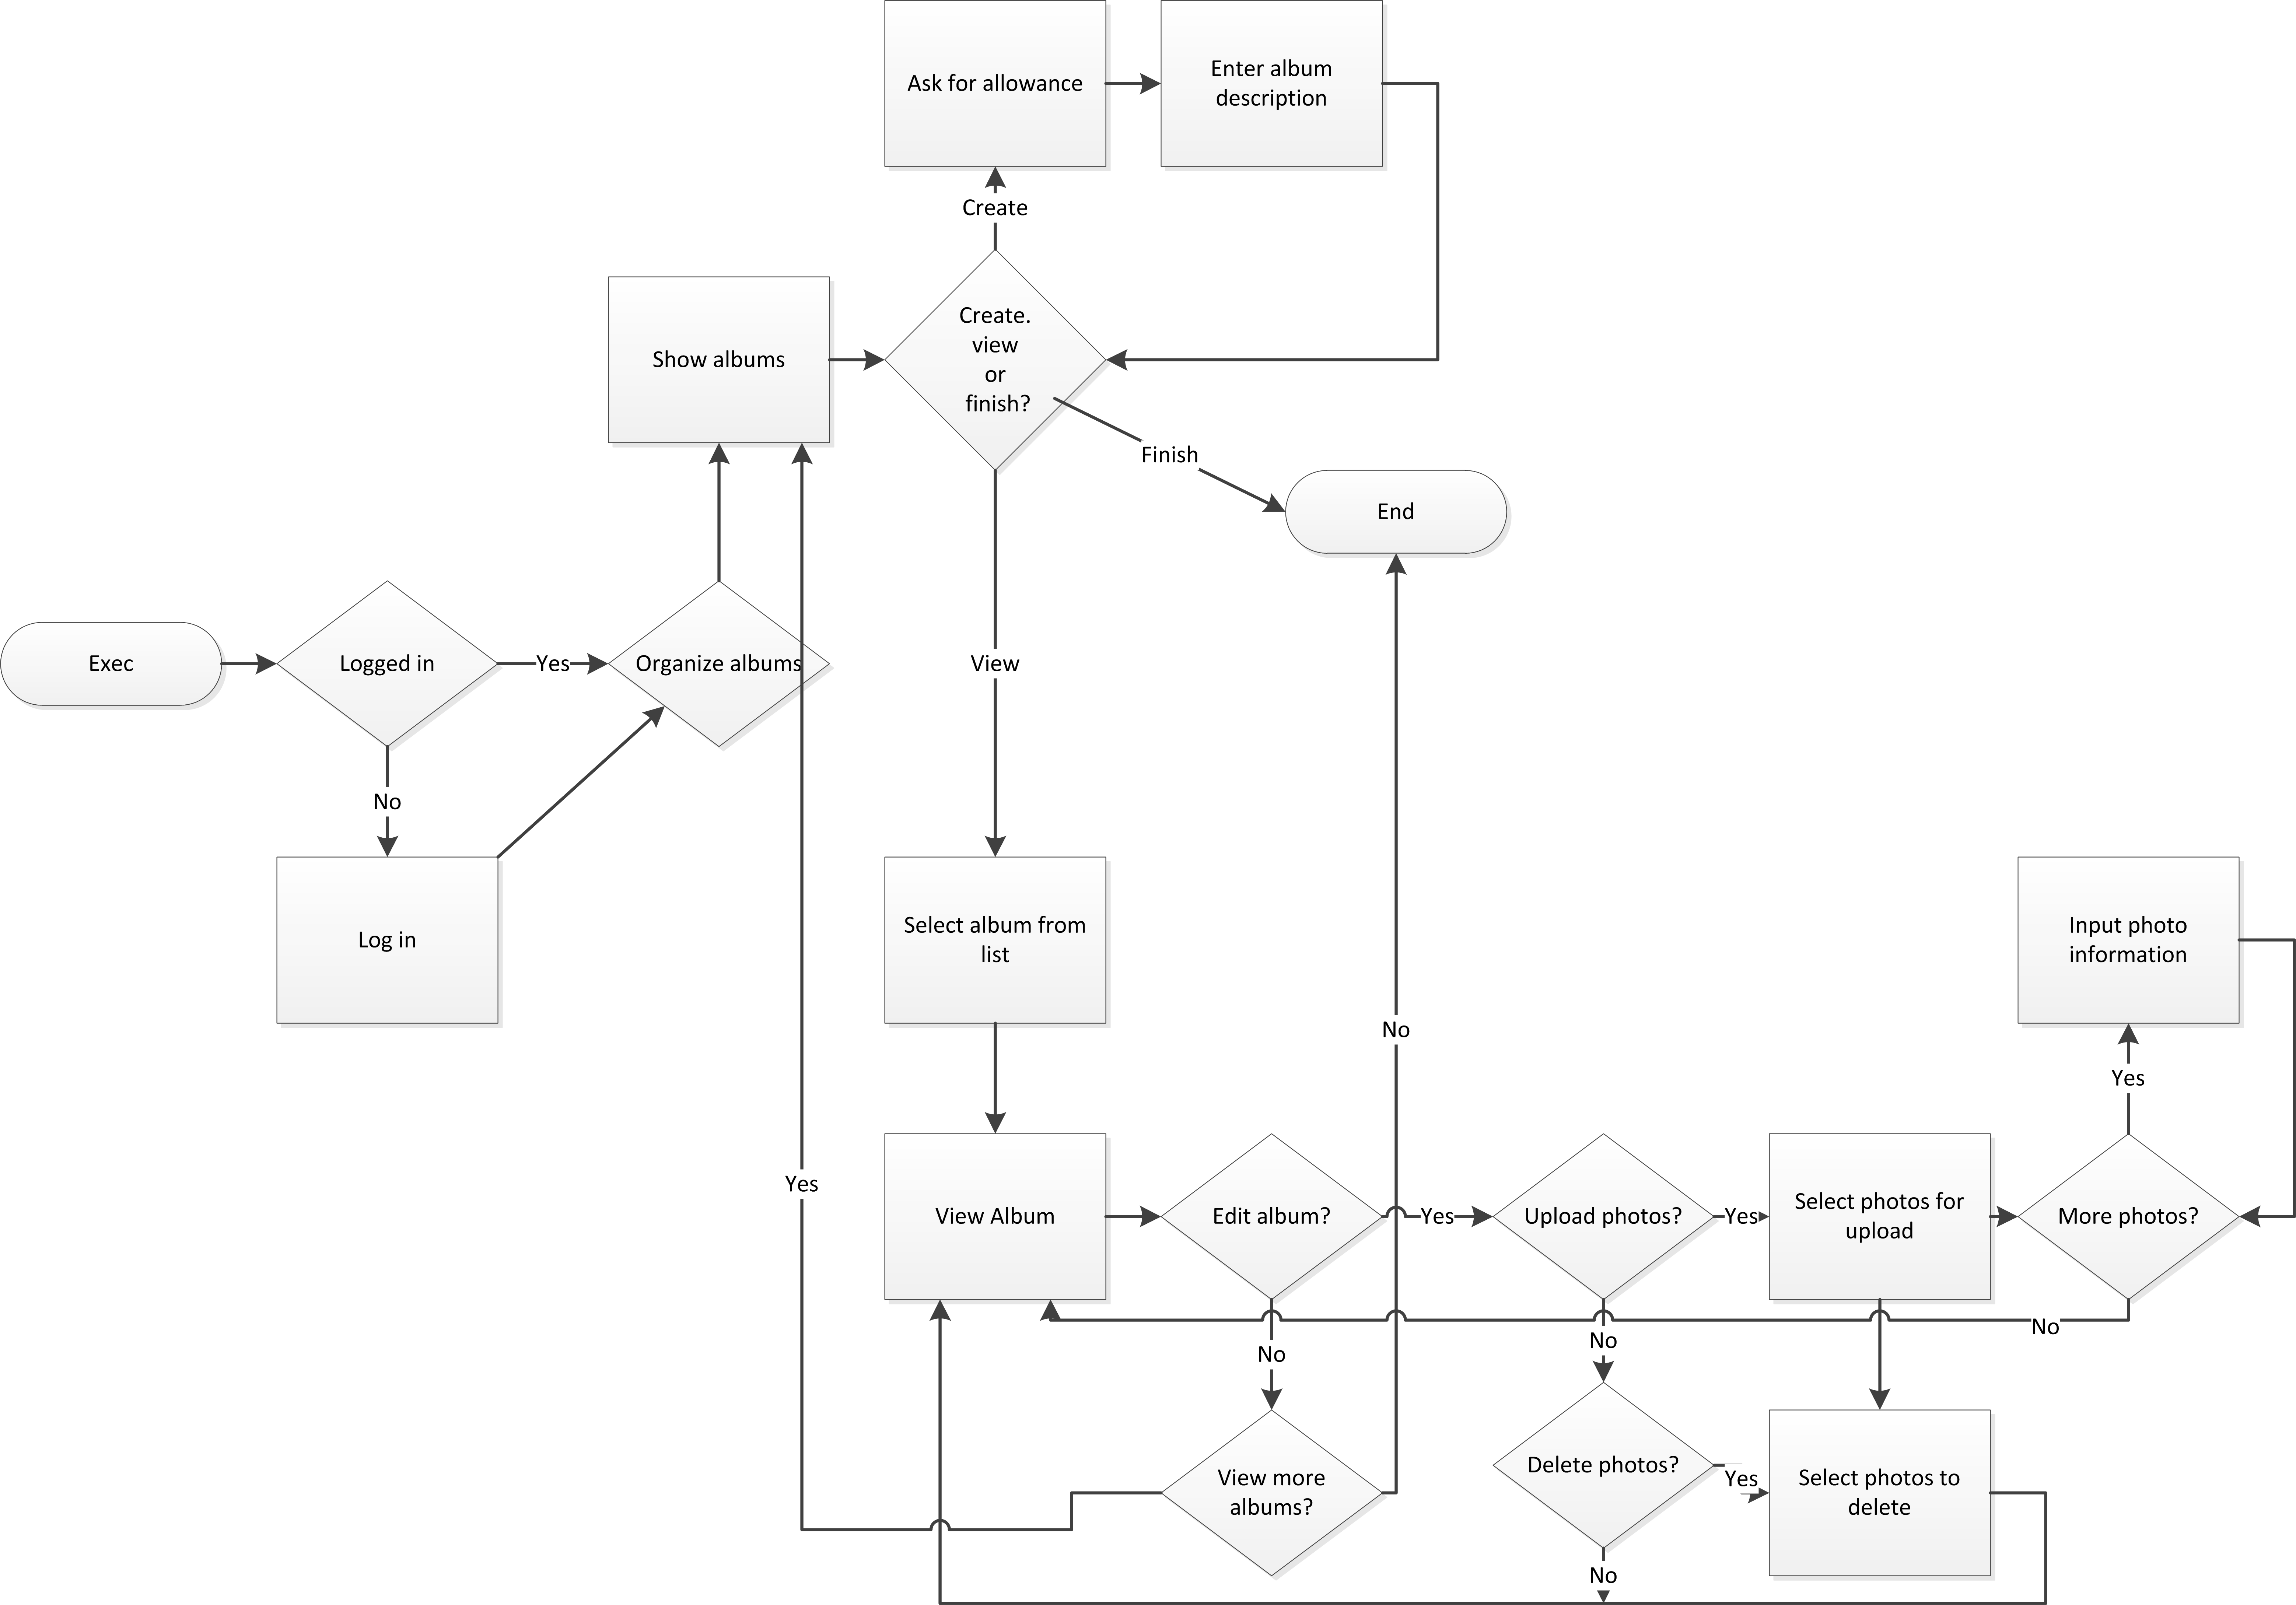
\includegraphics[scale=.75]{img/execUseCaseFE6_organize.png}
\label{fig:execUseCaseFE6_organize}
\end{sidewaysfigure}
\FloatBarrier

\newpage

\newpage

\FloatBarrier
\begin{sidewaysfigure}[h]
\centering
\caption{Brother Use Case Flowchart for FE-6}
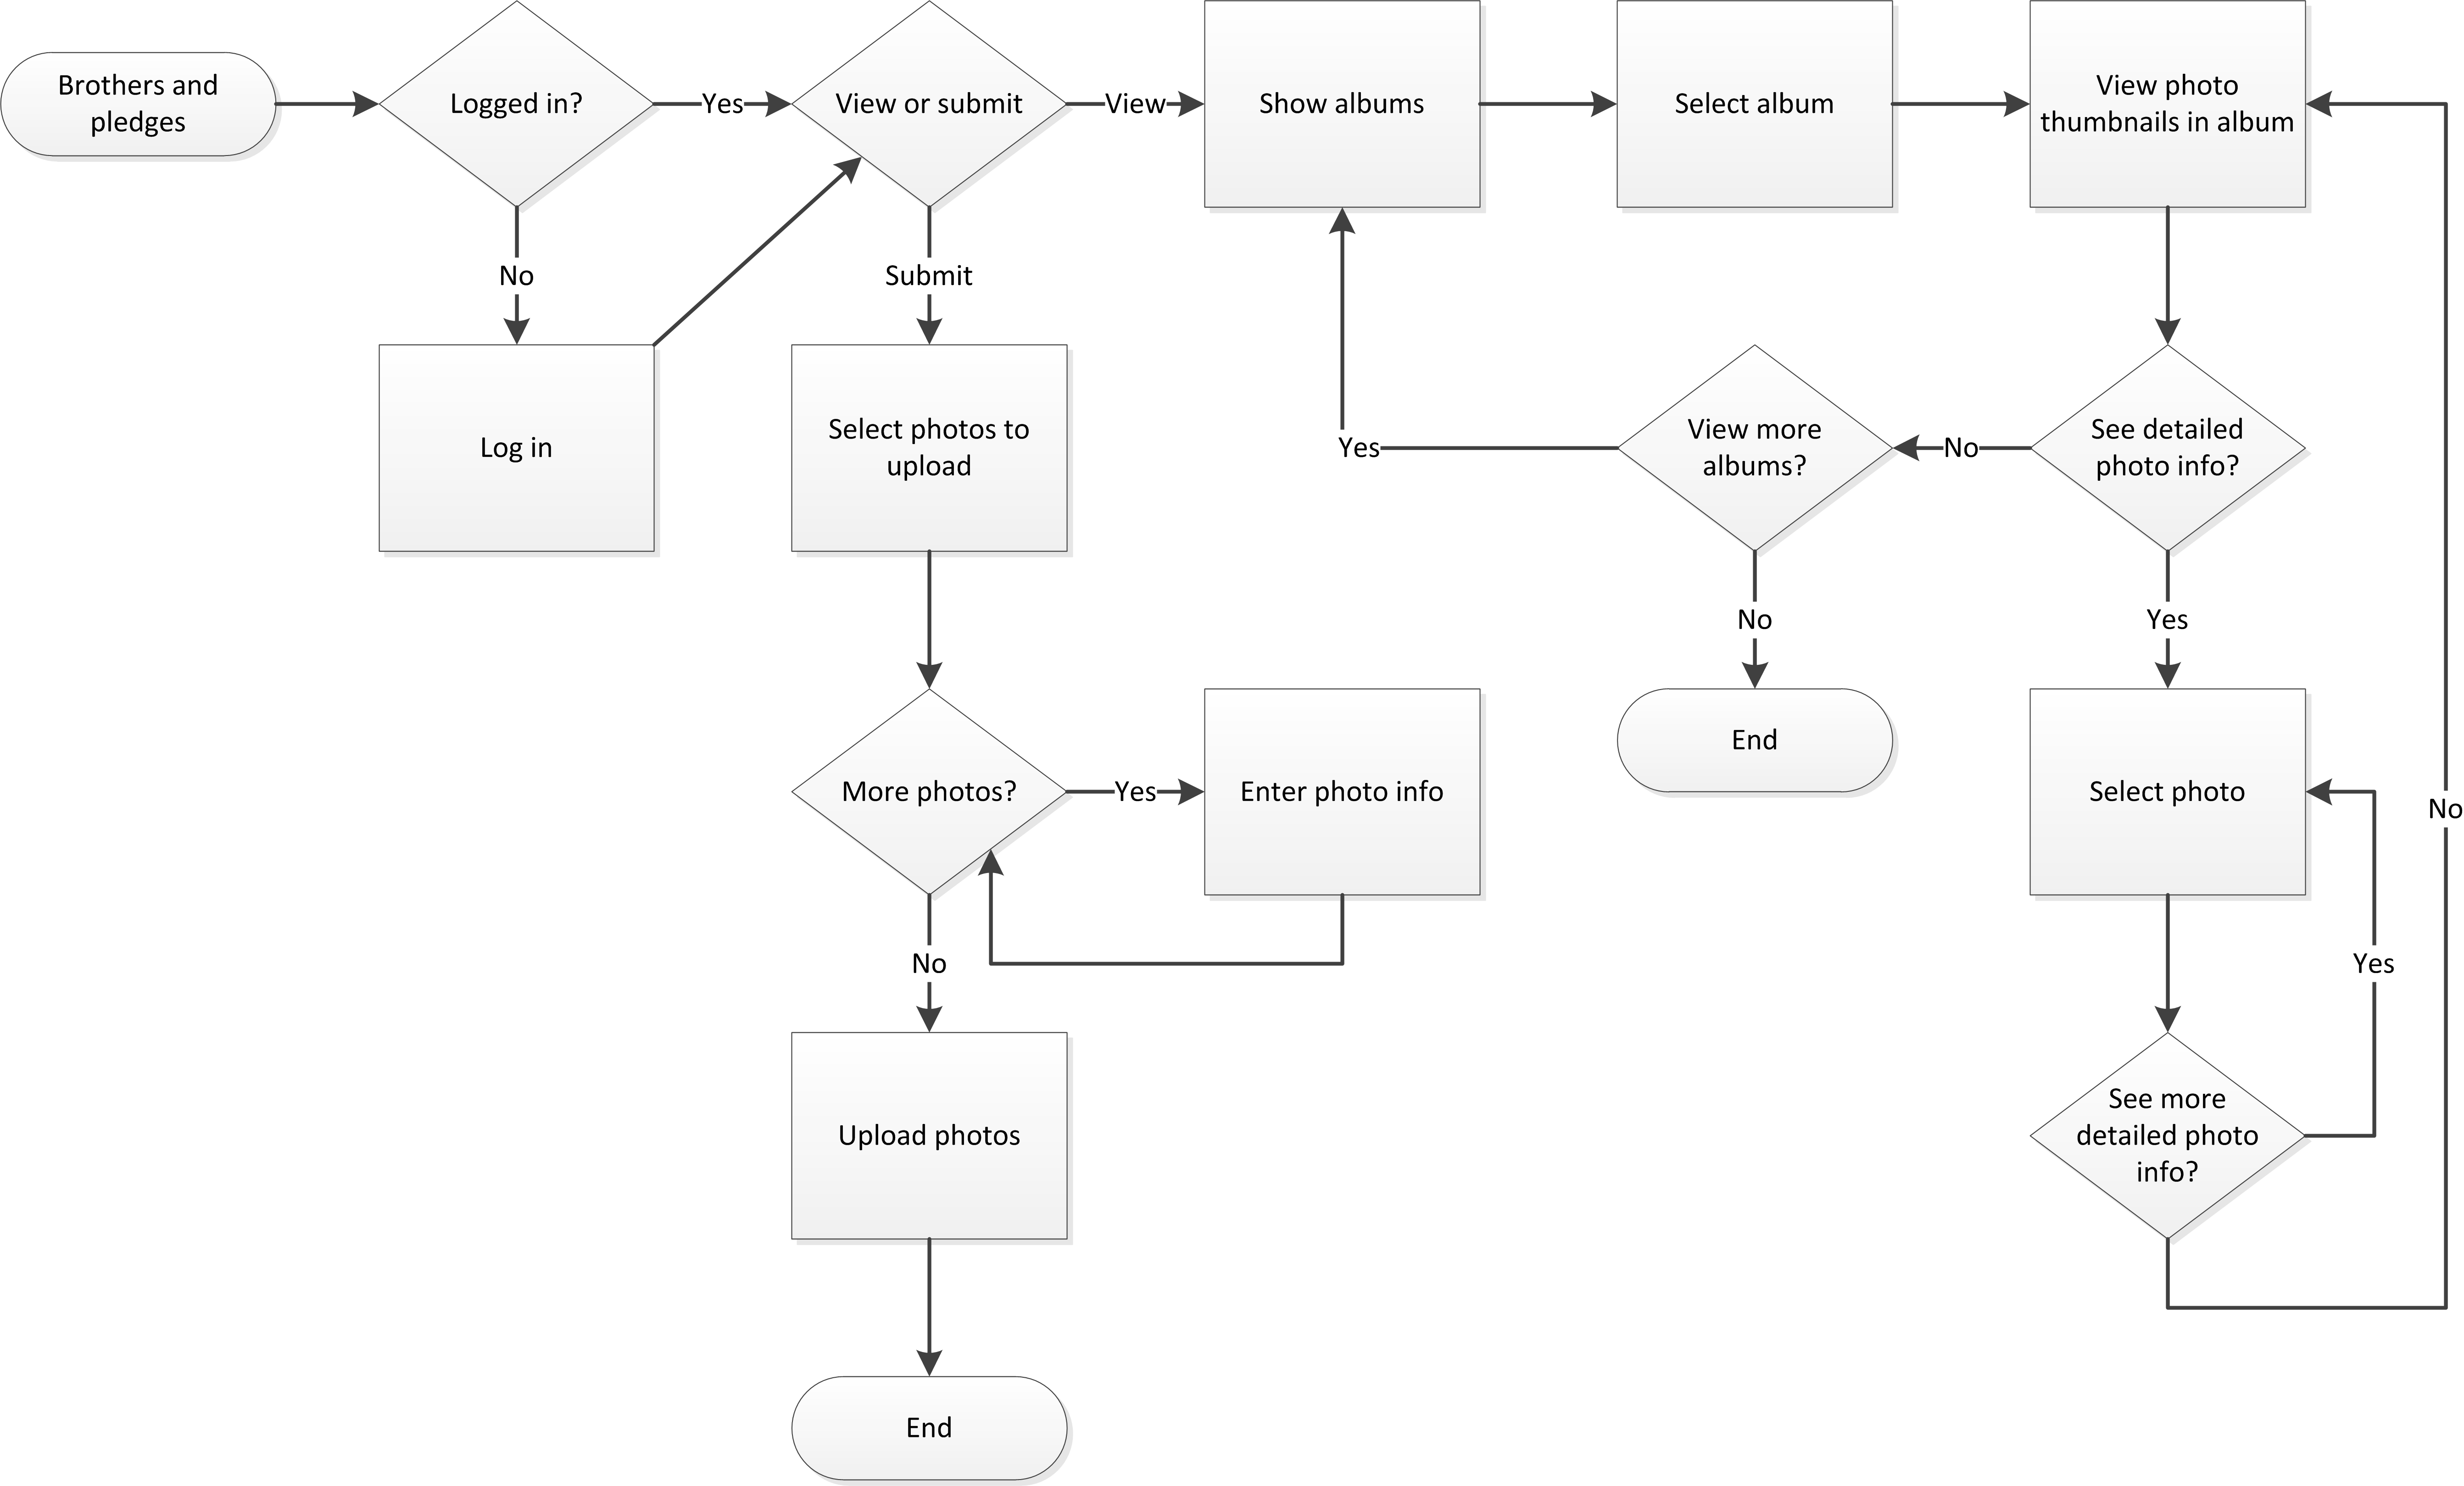
\includegraphics[scale=.75]{img/brotherUseCaseFE6.png}
\label{fig:brotherUseCaseFE6}
\end{sidewaysfigure}
\FloatBarrier

\newpage

\subsubsection{Requirements}

\begin{tabular}{lp{8cm}}
\req{32} & Exec members shall be able to create new photo albums \\
\req{32.1} & Exec members shall be able to add a title to new photo
albums\\
\req{32.2} & Exec members shall be able to add a description to photo albums\\
\req{33} & Exec members shall be able to add photos to albums \\
\req{33.1} & Exec members shall be able to add descriptions to photos\\
\req{34} & Exec members shall be able to review photo submissions from
members \\
\req{34.1} & Exec members shall be able to accept or reject photo submissions\\
\req{35} & Members shall be able to view existing albums and photos \\
\req{35.1} & Members shall be able to view album descriptions\\
\req{35.2} & Members shall be able to view photo descriptions\\
\req{36} & Members shall be able to submit photos to albums for review
\\
\req{36.1} & Members shall be able to submit photo descriptions\\
\end{tabular}

\subsection{FE-7: Track and report chapter statistics}

\subsubsection{Use case Diagram}

\newpage

\FloatBarrier
\begin{sidewaysfigure}[h]
\centering
\caption{Exec Use Case Flowchart for FE-7}
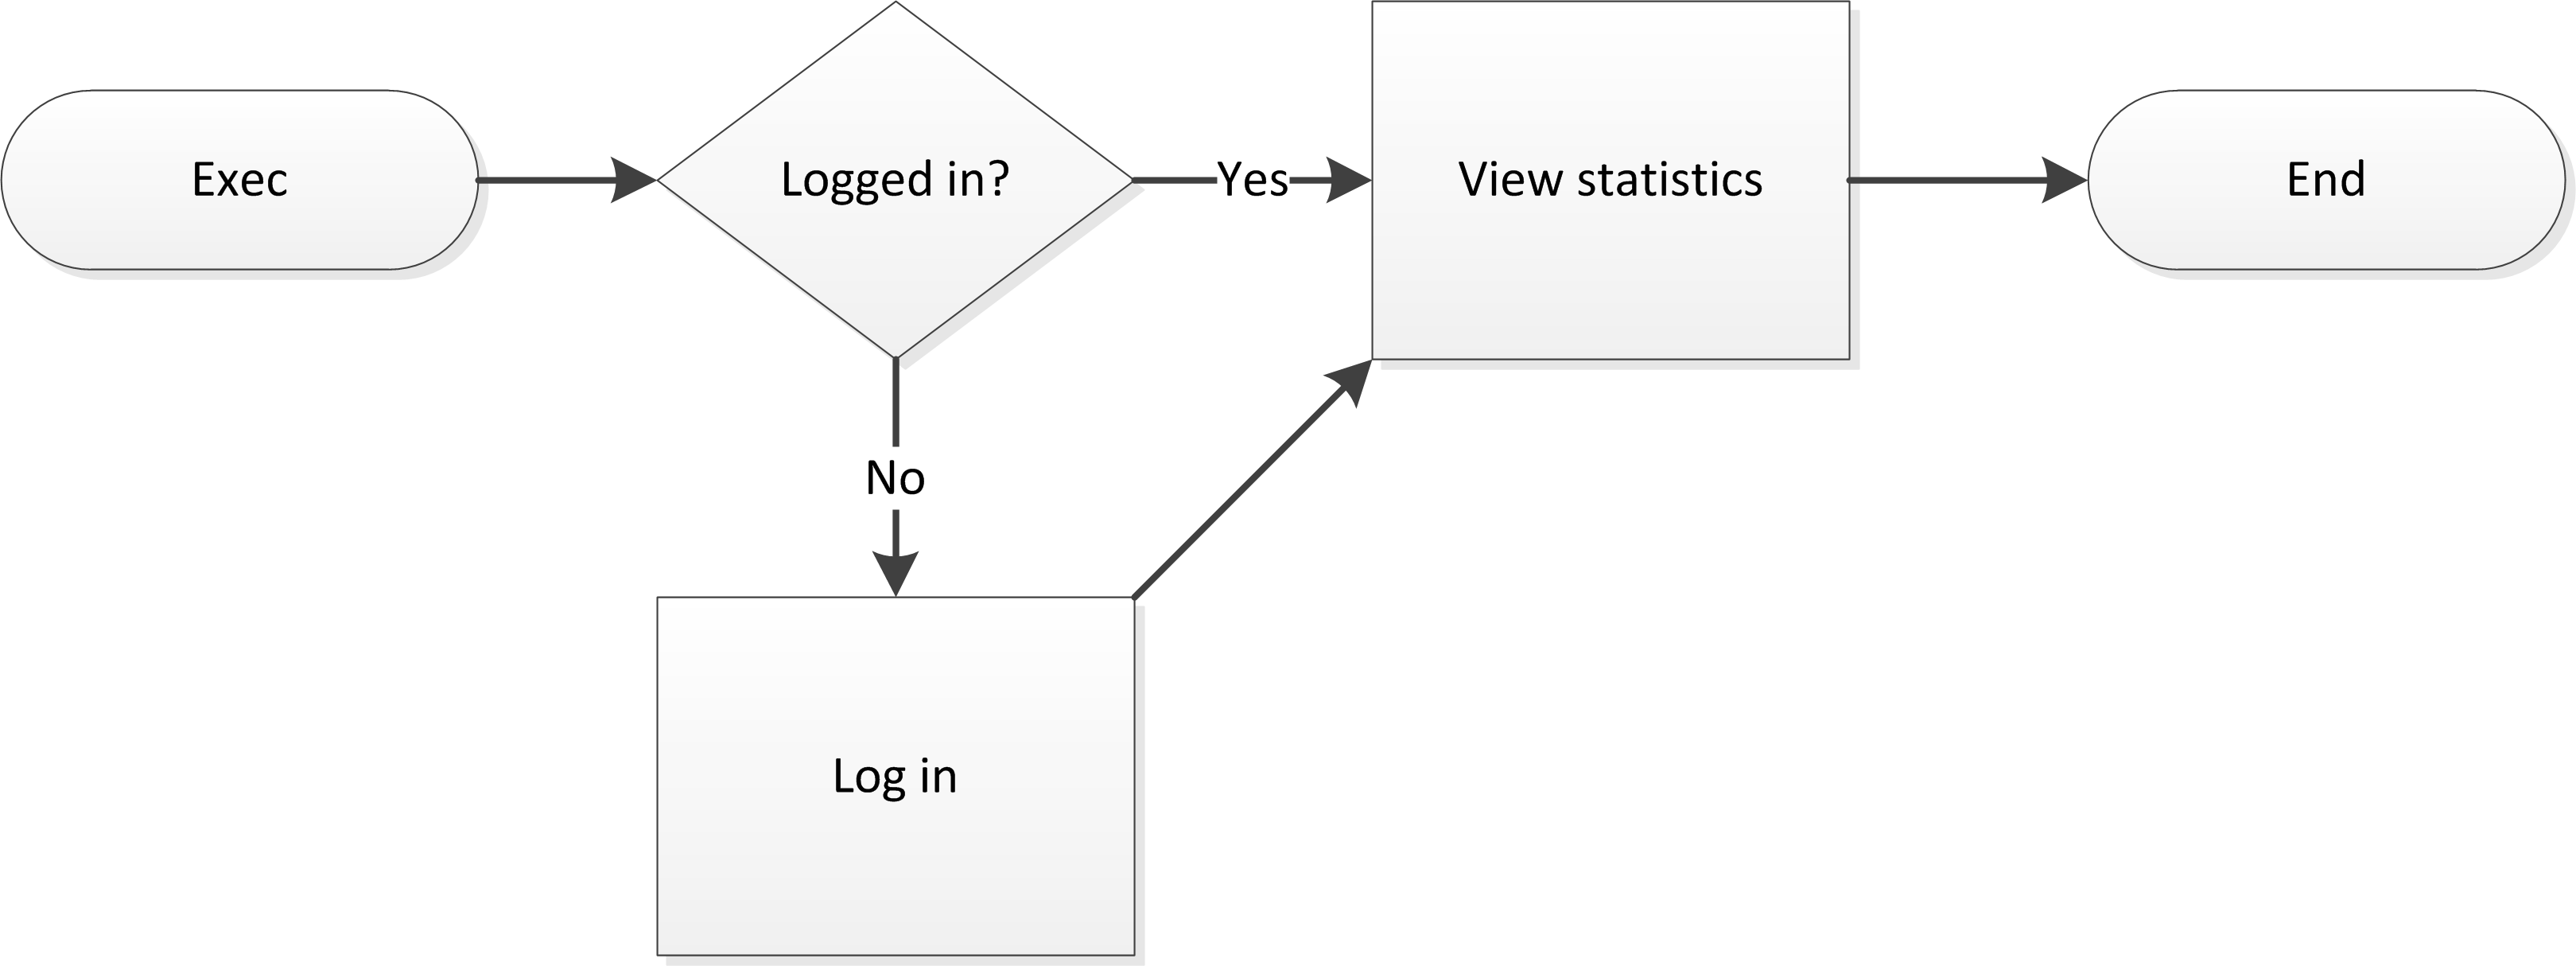
\includegraphics[scale=.75]{img/execUseCaseFE7.png}
\label{fig:execUseCaseFE1}
\end{sidewaysfigure}
\FloatBarrier

\newpage

\subsubsection{Requirements}

\begin{tabular}{lp{8cm}}
\req{37} & Exec members shall be able to view statistics \\
\req{37.1} & Exec members shall be able to view the number of each
type of contract signed \\
\req{37.2} & Exec members shall be able to view the number of members
who have completed their contract\\
\req{37.3} & Exec members shall be able to view the total number of
service hours completed by the chapter\\
\req{38} & Exec members shall be able to export information into an
offline format\\
\end{tabular}

\section{Additional Requirements}

\subsection{Performance}

\begin{tabular}{lp{8cm}}
\req{39} & Website shall be able to handle 20 simultaneous connections\\
\end{tabular}

\subsection{Security}

\begin{tabular}{lp{8cm}}
\req{40} & User login pages shall be encrypted\\
\req{41} & User passwords shall be encrypted before being stored\\
\end{tabular}

\end{document}